\documentclass{article}
\usepackage[left=0.5in,top=0.5in,right=0.5in,bottom=0.5in]{geometry}
\usepackage[english]{babel}
\usepackage[utf8]{inputenc}
\usepackage[table]{xcolor}
\usepackage{amssymb,amsmath,amsthm}
\usepackage{changepage,threeparttable}
\usepackage{booktabs,multirow}
\usepackage{graphicx}
\usepackage{soul}
\def\R#1#2{\(#1_{\text{\tiny#2}}\)}
\graphicspath{{./images/}}
\title{Lab 6: The Impedance of Capacitors}
\author{Philip Kim}
\date{\today}
\begin{document}
\maketitle
\vspace*{-1cm}
\begin{table}[!htp]\centering
  \subsection*{Part 1}
  \begin{tabular}{|c|c|c|c|c|c|c|c|c|c|c|}\hline
  \multicolumn{11}{|c|}{\textbf{Table 1: Impedance of a Capacitor}} \\\hline
  C & R & \R{V}{RC} & \R{V}{R} & V/DIV for \R{V}{R} & \R{f}{gen} & \R{f}{osc} & \R{I}{R} & \R{V}{C} & \R{X}{C,exp} & \R{X}{C,the} \\\hline
  0.22\(\mu F\) & 1k\(\Omega \) & 3.97V & 3.08V & 2V & 523Hz & 538.793Hz & 0.0031 & 2.5049V & 993.6\(\Omega \) & 1383.2\(\Omega \) \\\hline
  0.33\(\mu F\) & 1k\(\Omega \) &  &  &  &  &  &  &  &  &  \\\hline
  0.10\(\mu F\) & 1k\(\Omega \) &  &  &  &  &  &  &  &  &  \\\hline
  0.47\(\mu F\) & 1k\(\Omega \) &  &  &  &  &  &  &  &  &  \\\hline
  0.68\(\mu F\) & 1k\(\Omega \) &  &  &  &  &  &  &  &  &  \\\hline
  1.00\(\mu F\) & 1k\(\Omega \) &  &  &  &  &  &  &  &  &  \\\hline
  \end{tabular}
  \begin{center}
    \subsection*{Picture \R{R}{RC} \& \R{R}{C}}
    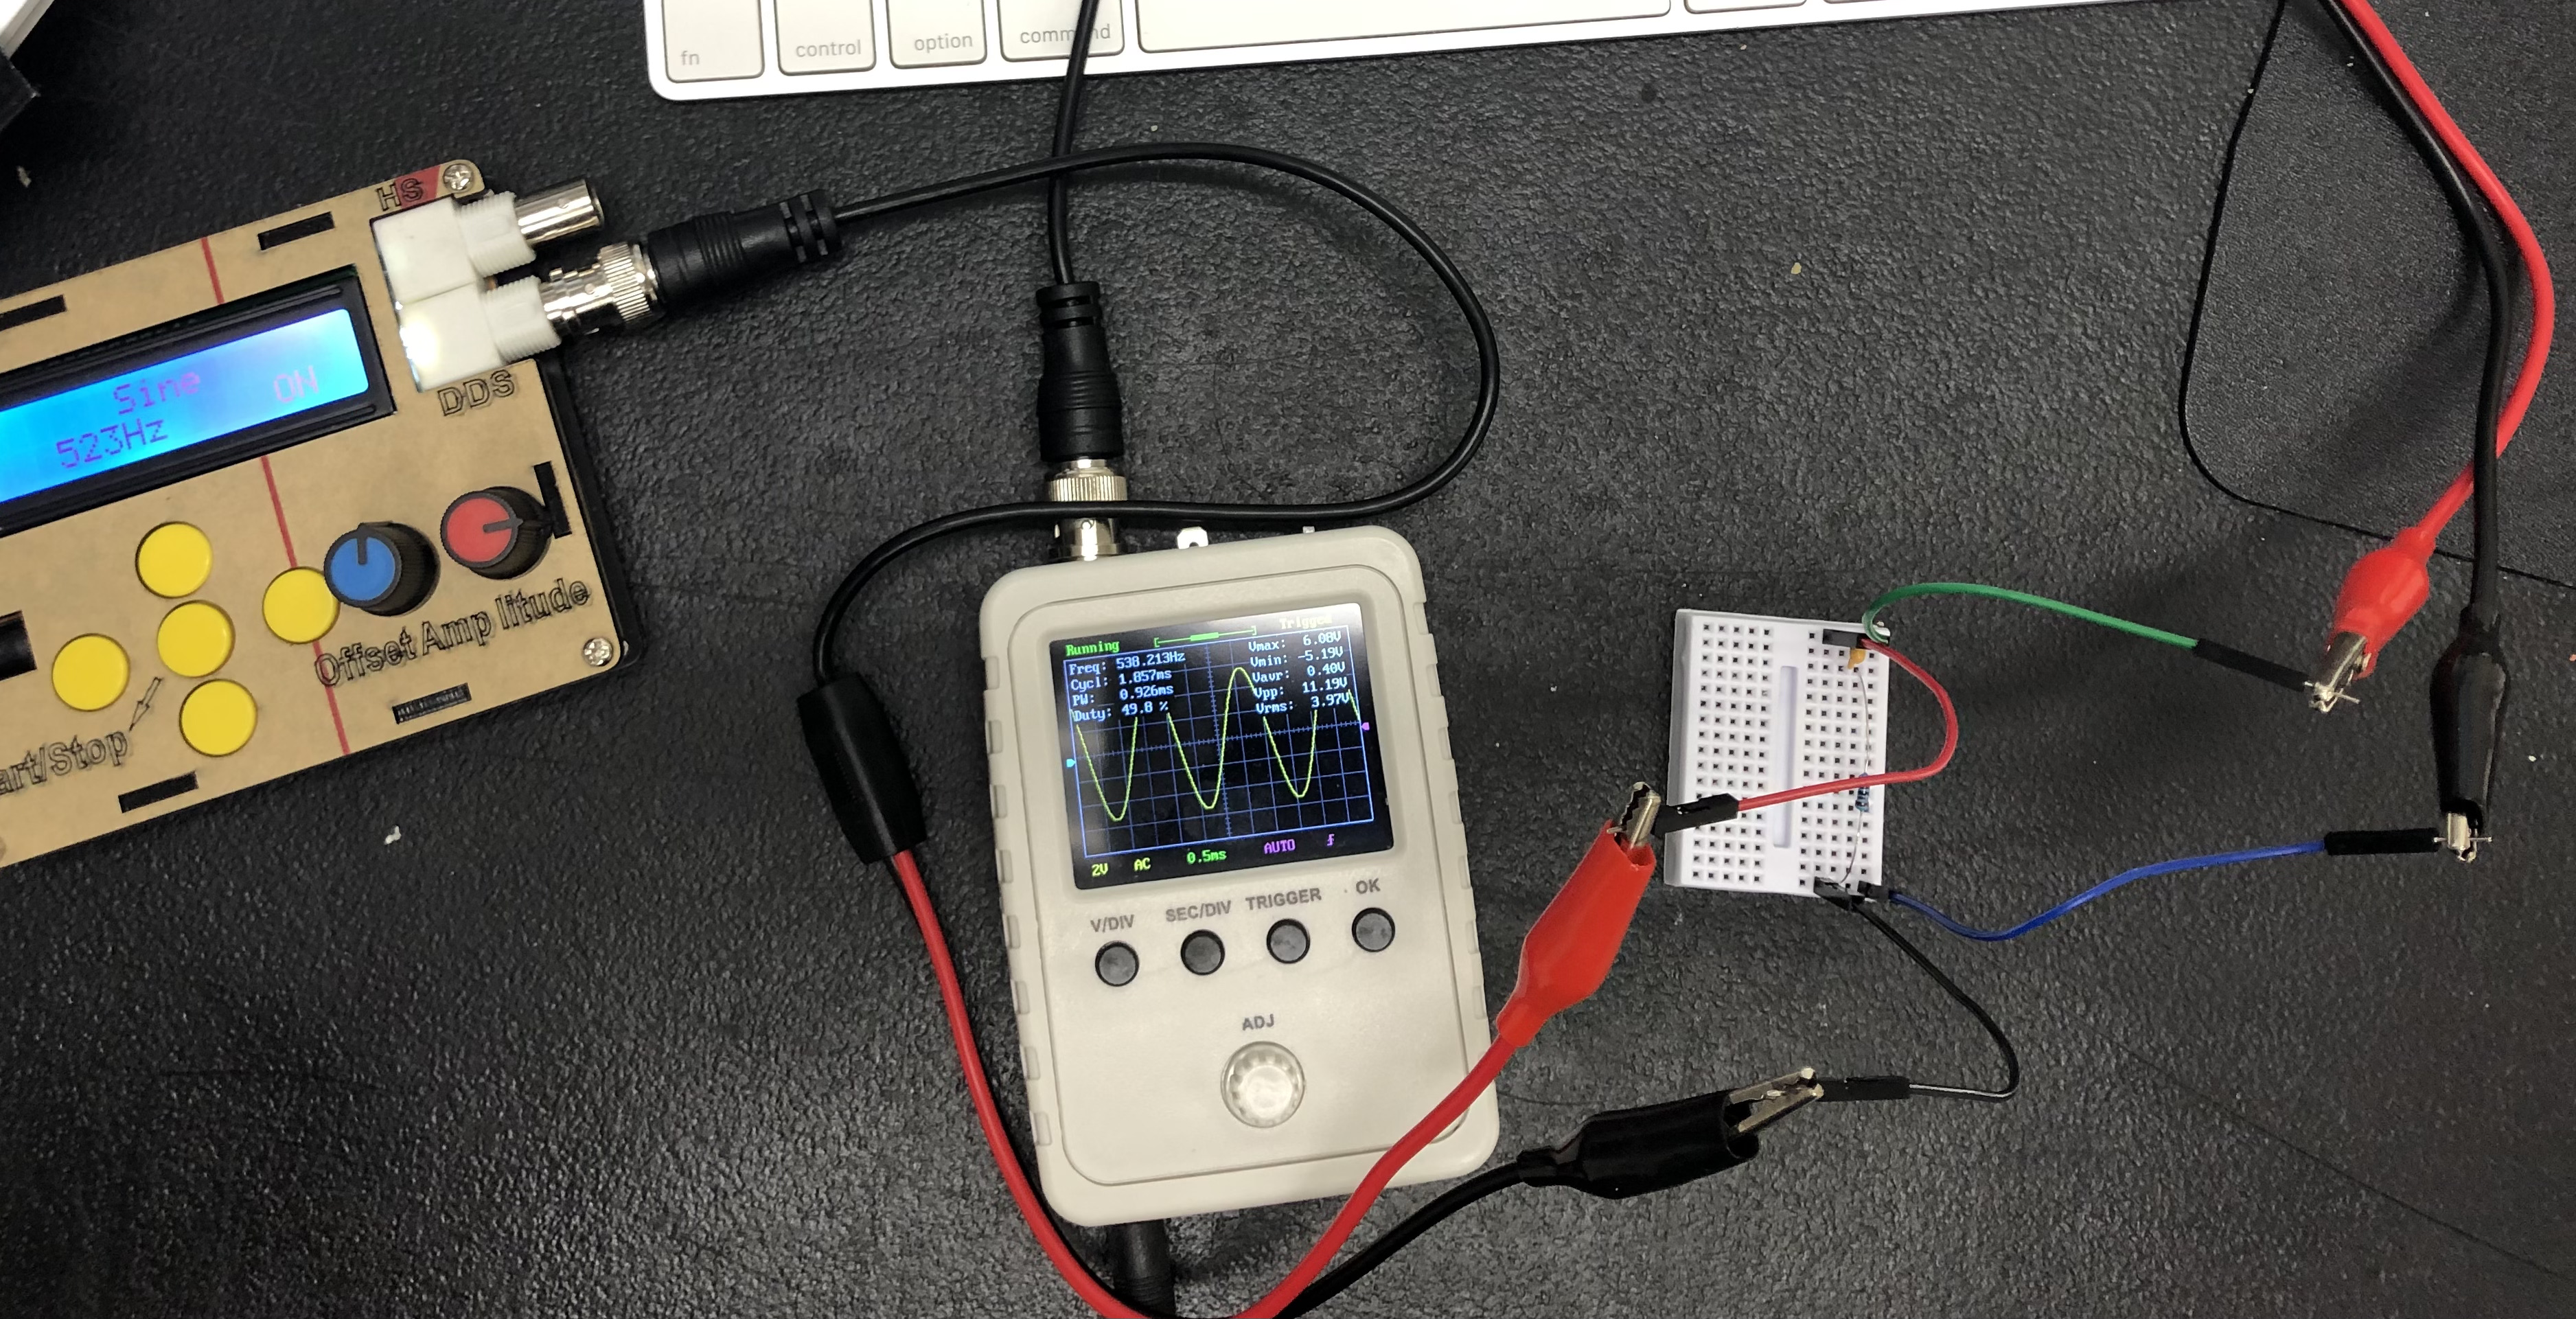
\includegraphics[width=8cm,height=4.5cm]{Vrc.jpeg}
    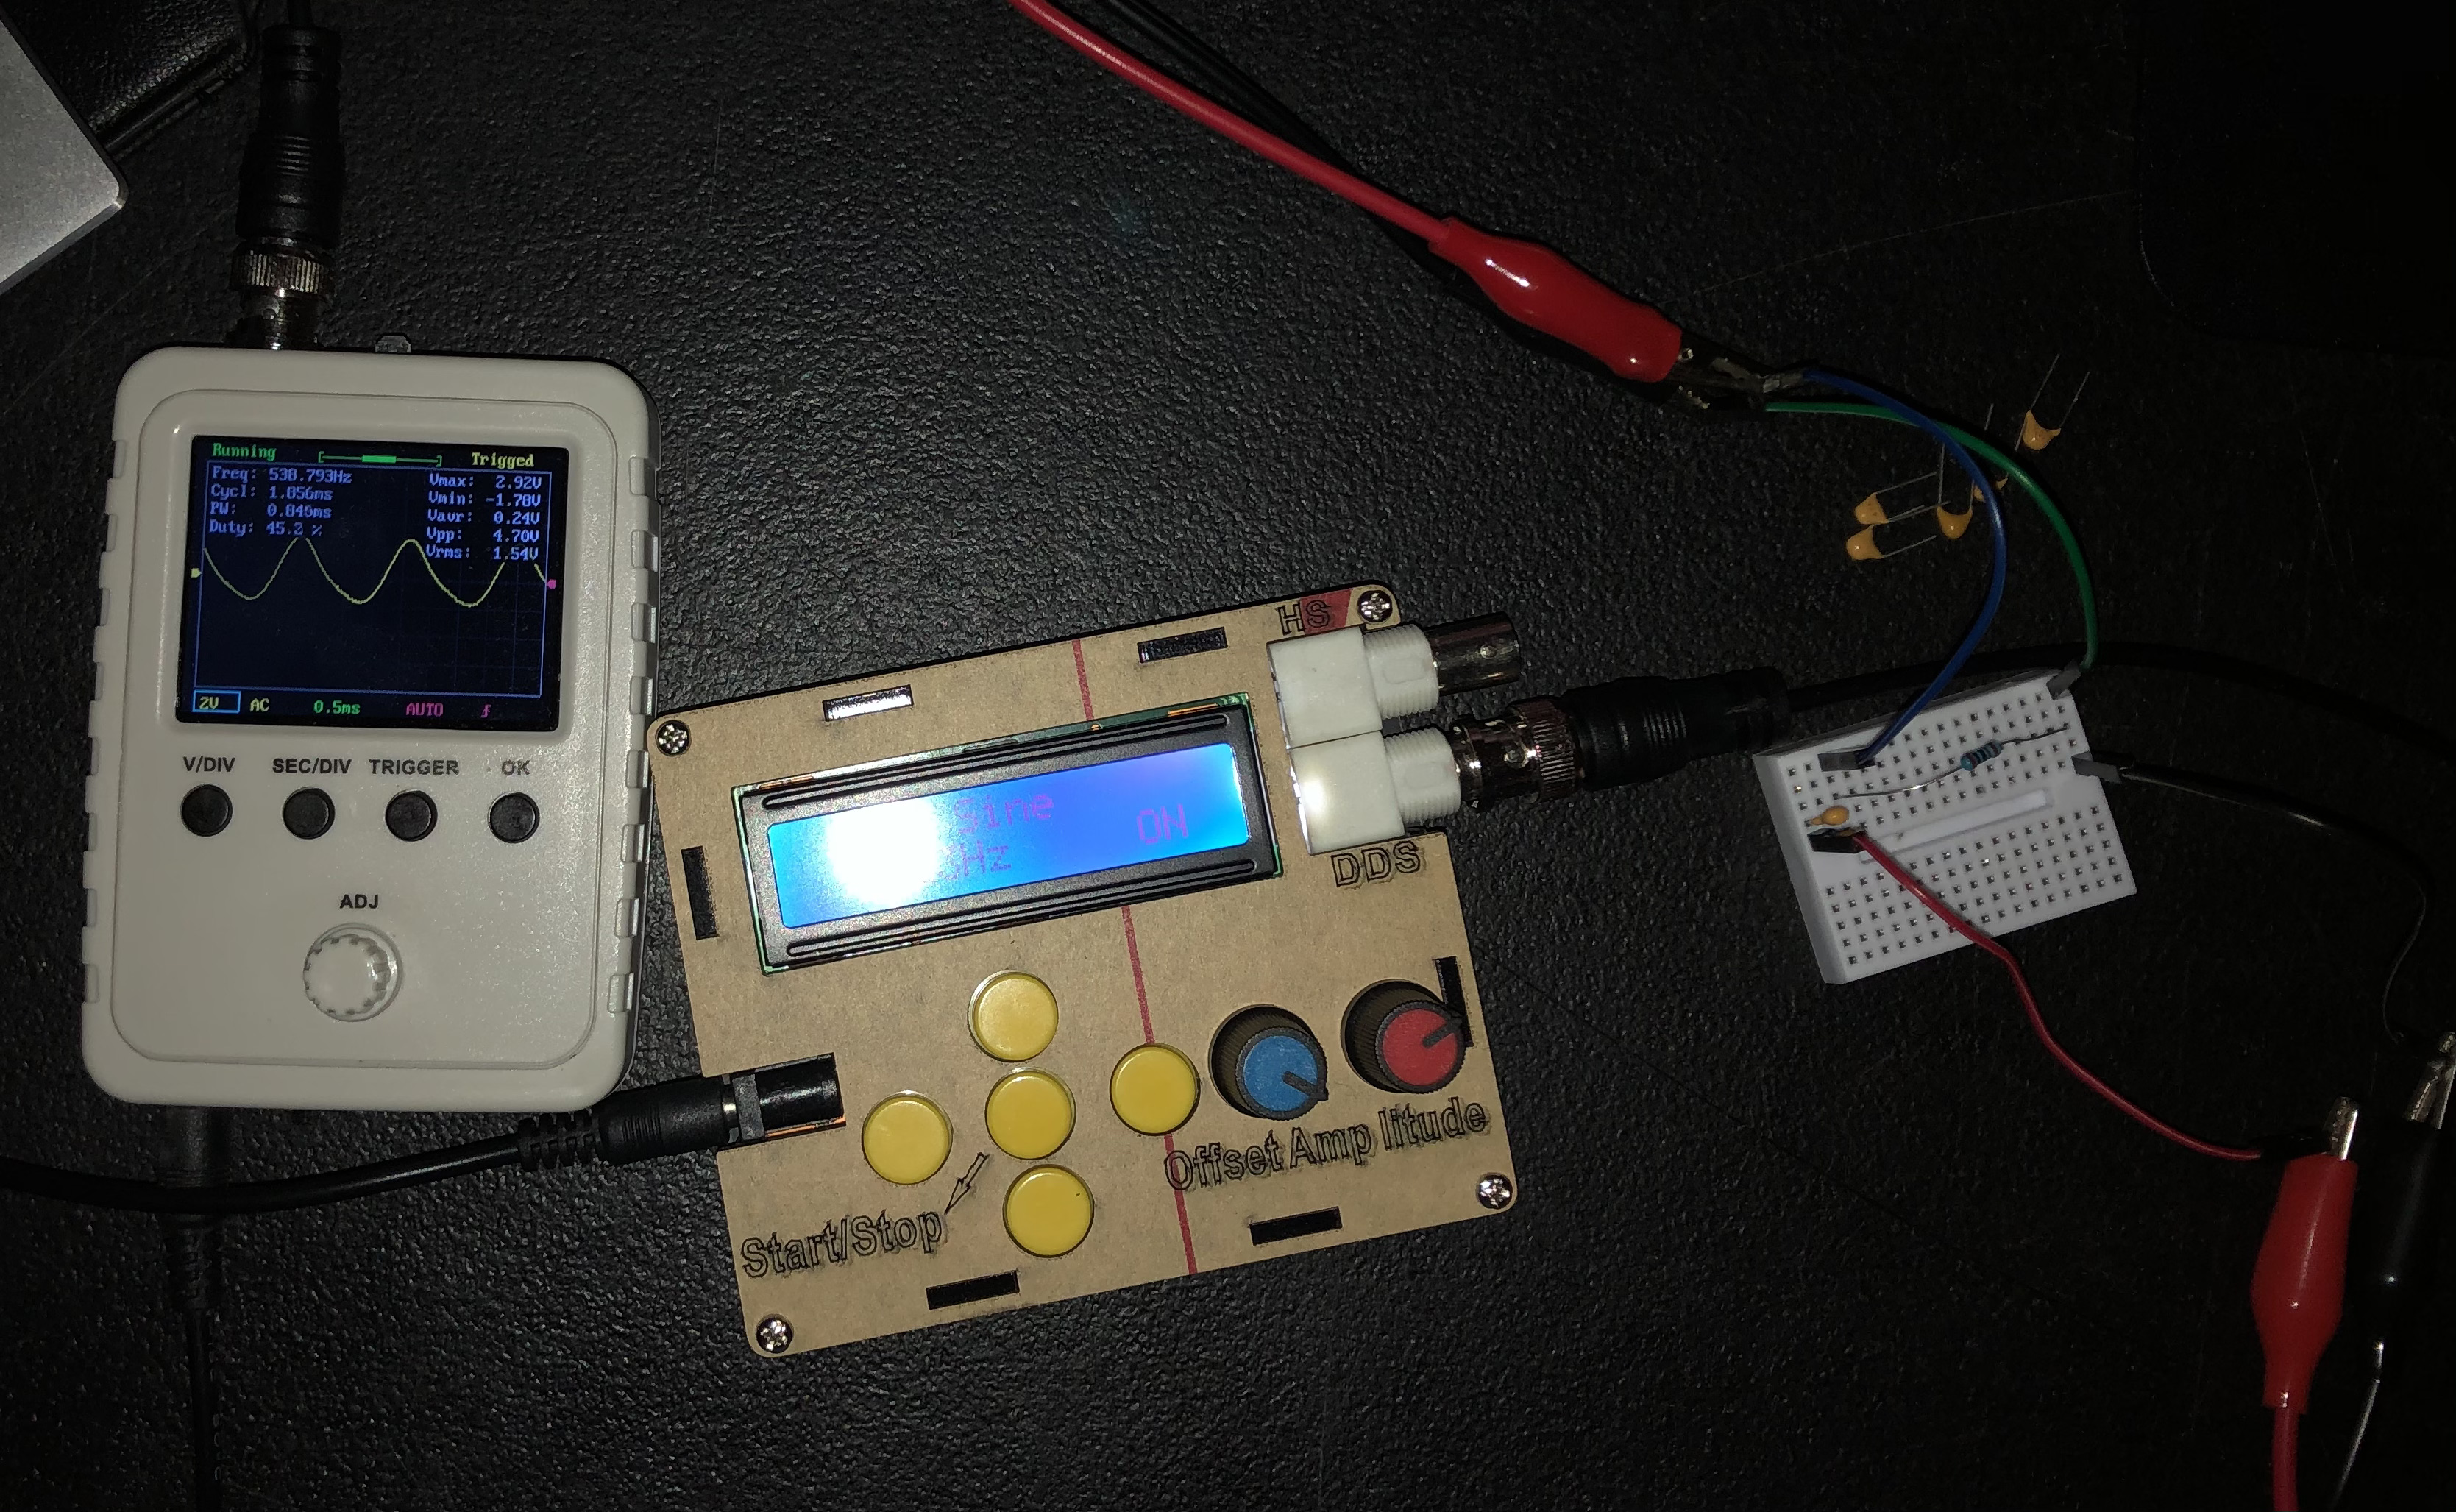
\includegraphics[width=8cm,height=4.5cm]{Vr.jpeg}
    \subsection*{Graph 1}
    % 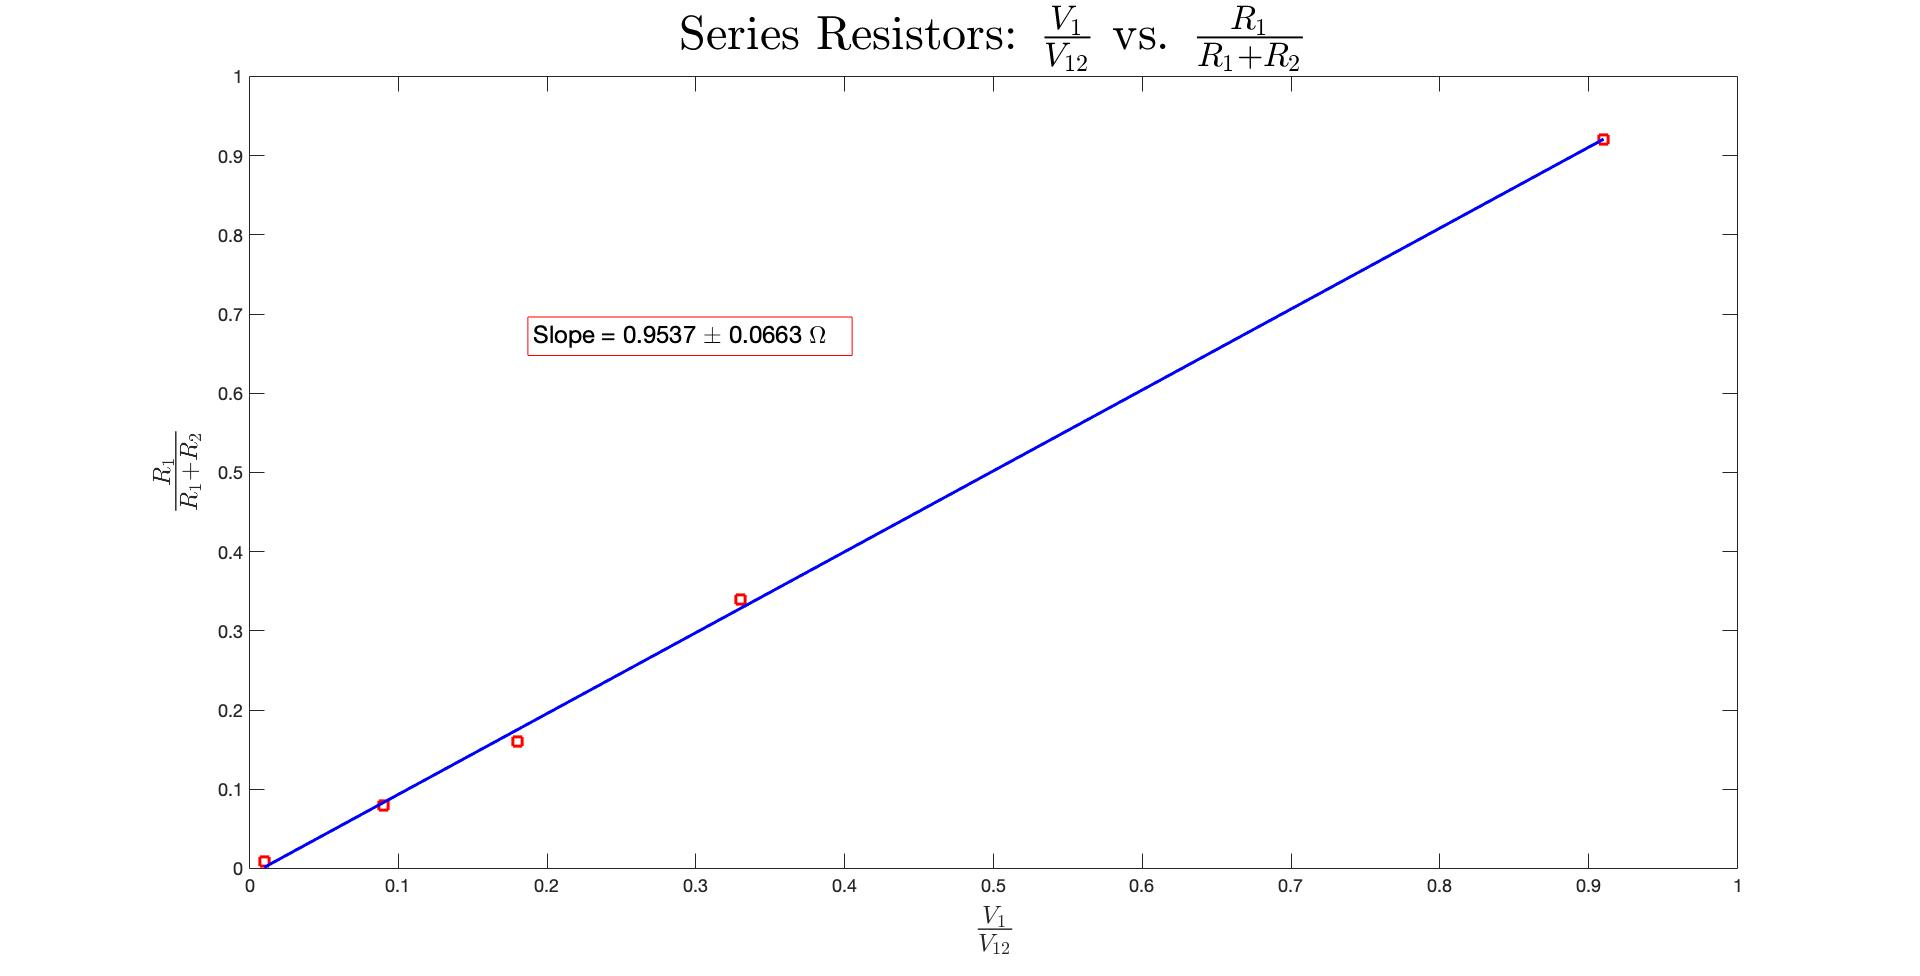
\includegraphics[scale=0.2]{series.jpg}
    \subsection*{Graph 2}
    \subsection*{Discussion 1}
    \begin{enumerate}
      \item What slope do you find for graph 2 and how does it compare to your expectation?
      \begin{itemize}
        \item
      \end{itemize}
      \item What does a deviation from the linear fit indicate? How would you correct for the ones with the largest error?
      \begin{itemize}
        \item
      \end{itemize}
    \end{enumerate}
  \end{center}
\end{table}
\end{document}